%############################# Anhang #################################
\appendix
%\chapter{Mathematischer Anhang}
%\chapter{Programmcodes}
\chapter{Appendix}

Write here small introduction to appendix! %TODO
\clearpage
\section{Complete Feature List}
\begin{table}[ht]
    \centering
    \small
    \renewcommand{\arraystretch}{1.3}
    \begin{tabular}{@{}cccc@{}}
        NoCustomers            & width-height-min   & width-W-min   & volume-WLH-min   \\
        NoItems                & width-height-max   & width-W-max   & volume-WLH-max   \\
        Rel Volume             & width-height-mean  & width-W-mean  & volume-WLH-mean  \\
        Rel Weight             & width-height-std   & width-W-std   & volume-WLH-std   \\
        Rel Total Length Items & length-height-min  & length-L-min  & height-area-min  \\
        Rel Total Width Items  & length-height-max  & length-L-max  & height-area-max  \\
        Rel Total Height Items & length-height-mean & length-L-mean & height-area-mean \\
        Fragile Ratio          & length-height-std  & length-L-std  & height-area-std  \\
        Fragile Sequence       & width-length-min   & height-H-min  & area-AREA-min    \\
        Volume Balance         & width-length-max   & height-H-max  & area-AREA-max    \\
        Volume Distribution    & width-length-mean  & height-H-mean & area-AREA-mean   \\
        Weight Distribution    & width-length-std   & height-H-std  & area-AREA-std    \\
    \end{tabular}
    \caption{Complete feature list.}
    \label{tab:complete_features_list}
\end{table}

\clearpage
\section{Random Route Generation}
\label{chap:appendix:RRG}
This appendix chapter helps understanding the algorithm used for the generation of random routes. The complete algorithm
is depicted in Figure~\ref{fig:flowchart_randomRouteGeneration} and the following Algorithm~\ref{alg:appendix:check_single_tour}
is used to check the volume and weight limit of one single tour.
\begin{algorithm}[ht]
    \caption{Check volume and weight limit}
    \label{alg:appendix:check_single_tour}
    \begin{algorithmic}[1]\onehalfspacing
        \Require{Volume limit $V$, Weight limit $Q$, Uniform distribution $\mathcal{U}(a,b)$}
        \Procedure{Feasible}{$\text{Route}\,R,\, \text{Lower Threshold}\,\delta$}
        \State{Get subset of customers $S$ from route $R$}
        \State{$V^* \gets V \cdot \mathcal{U}(\delta,\,1)$} \Comment{Individual bounds for each single route}
        \State{$Q^* \gets Q \cdot \mathcal{U}(\delta,\,1)$}
        \If{$q(S)\le Q^* \, \wedge \, v(S)\le V^*$} \Comment{Check feasibility}
        \State{\textbf{return} true}
        \Else
        \State{\textbf{return} false}
        \EndIf
        \EndProcedure
    \end{algorithmic}
\end{algorithm}

As the following flowchart contains a lot of information and many different symbols the used terms are explained in
the following. The parameters $\mathcal{I}$, $\alpha$, $\beta$, $\gamma$ and $\delta$ were alredady described in
Section~\ref{sec:DataRetrieval}.

\begin{itemize}\singlespacing
    \item $\mathcal{G}$: Set of found routes
    \item $i$: Current instance
    \item $n$: Numbers of customers / Length of route
    \item $n_{max}$: Maximum numbers of customers in instance $i$
    \item $c$: Counter for inner loops finding no tour
    \item $t$: Iteration counter for inner loop (no function!)
    \item $k$: Counter for found tours in the inner loop
    \item $a$: Counter for failed attempts to find a feasible tour
    \item $x$: Counter for breakups
    \item SuccessBool: Boolean, if at least one route was found in inner loop
    \item BreakBool: Boolean for interrupting current instance $i$, when for one customer number $n$ no route could be found
\end{itemize}



\begin{figure}[ht]
    \centering
    \footnotesize
    \begin{tikzpicture}[
            scale = 0.983, transform shape,node distance=7mm and 11mm,
            >=Latex,
            % Styles
            startstop/.style   = {rectangle, draw, align=center, minimum width=22mm, minimum height=6mm},
            process/.style     = {rectangle, draw, align=center, minimum width=30mm, minimum height=6mm},
            decision/.style    = {diamond, draw, aspect=2, inner sep=1pt, align=center, minimum width=40mm,minimum height=20mm},
            io/.style          = {trapezium, trapezium left angle=60, trapezium right angle=120, draw, align=center, minimum height=6mm},
            connector/.style   = {circle, draw, inner sep=1pt},
            line/.style        = {->}
        ]

        % Nodes
        \node[startstop] (start) {Start RRG ($\mathcal{I}$, $\alpha$, $\beta$, $\gamma$, $\delta$)};
        \node[decision, below=of start] (forI) {$i\in\mathcal{I}$ left?};
        \node[process, left= of forI] (nextI) {Next $i$ \&\\ Save $\mathcal{G}$};
        \node[process, below=of forI] (initI) {$\mathcal{G}\gets\emptyset$\\$n_{\max}\gets \mathrm{MaxCustomers}(i)$\\BreakBool$\gets$False};
        \node[decision, below=5mm of initI] (forN) {$n=2\ \to\ n_{\max}$ left?};
        \node[decision, below=of forN] (exitOuter) {BreakBool?};
        \node[decision, right=of exitOuter] (breakDec) {$c \geq n \cdot \alpha$?};
        \node[startstop] at ($(breakDec.north |- forI.east)$) (end) {End RRG};
        \node[decision, below=of exitOuter] (forAlpha) {$t=1\ \to\ n\cdot\alpha$ left?};
        \node[decision, below=of forAlpha] (whileK) {While\\$k<\gamma$?};
        \node[decision, below=12 mm of whileK] (dup) {$R\in\mathcal{G}$?};
        % \node[process, bel=of dup] (drawThresh) {$Q^*\gets Q\cdot \mathcal{U}_\delta^1$\\$V^*\gets V\cdot \mathcal{U}_\delta^1$};
        \node[decision, right=of dup] (feasible) {Feasible($R$, $\delta$)?\\(See Alg.~\ref{alg:appendix:check_single_tour})};
        \node[process, above=10mm of feasible] (accept) {$\mathcal{G}\gets \mathcal{G}\cup\{R\}$\\SuccessBool$\gets$True};
        \node[decision, below= of feasible] (attemptCond) {$a\ge \beta$?};
        \node[process] at ($(dup.south |- attemptCond.west)$) (incX) {$x\gets x+1$};
        \node[process, left=of dup] (incC) {$c\gets c+1$};
        \node[decision] at ($(incC.south |- incX.west)$)  (breakCond) {$x\ge \gamma$ \& \\$\overline{\text{SuccessBool}}$?};
        \node[process] at ($(breakDec.north |- forN.east)$) (trueExit) {BreakBool$\gets$True};

        % Edges
        \draw[line] (start) -- (forI);
        \draw[line] (forI) -- node[pos=0.5, right]{yes}(initI);
        \draw[line] (forI) -- node[pos=0.5, above]{no}(end);
        \draw[line] (initI) -- (forN);
        \draw[line] (nextI.east)-- (forI.west);
        \draw[line] (forAlpha.east) -| node[pos = 0.25,above]{no}(breakDec.south);
        \draw[line] (breakDec.west) -- node[pos = 0.5,above]{no}($(breakDec.west)-(5mm,0)$) |- (forN.east);
        \draw[line] (breakDec) -- node[pos = 0.5,right]{yes}(trueExit);
        \draw[line] (trueExit) -- (forN);
        \draw[line] (whileK.west) -- ($(whileK.west)-(10mm,0)$) coordinate (bend) node[pos = 0.5,above]{no} |- (forAlpha.west);

        \draw[line] (forN.south) --  node[pos=0.5, right]{yes}(exitOuter.north);
        \draw[line] (forN.west) -|  node[pos=0.25, above]{no}(nextI.south);
        \draw[line] (exitOuter.west) -| node[pos=0.25, above]{yes} (nextI.south);

        \draw[line] (exitOuter) -- node[pos=0.5, right, align=left]{no\\$c \gets 0$} (forAlpha);

        \draw[line] (forAlpha) -- node[pos=0.5, right, align=left]{$k,a,x\gets 0$\\ SuccessBool$\gets$False} (whileK);
        \draw[line] (whileK) --node[pos=0.5, right, align=left]{yes \\ $R\gets \mathrm{RandomTour}(i,n)$} (dup);
        \draw[line] (dup) -- node[pos=0.5, below]{no}(feasible);
        \draw[line] (dup) -- node[pos=0.5, right]{yes}(incX);
        \draw[line] (incX) -- (breakCond);
        %\draw[line] (breakCond) -- node[pos=0.25, below right]{no}(whileK);
        \draw[line] (breakCond) |- node[pos=0.5, left]{no}($(incX.south)-(0,10mm)$) -| ($(attemptCond.east)+(10mm,0)$) coordinate (bend)|- (whileK);
        \draw[line] (breakCond) -- node[pos=0.5, left]{yes} (incC);
        \draw[line] (incC) |- (forAlpha);

        \draw[line] (feasible) -- node[pos=0.5, left]{yes}(accept);
        \draw[line] (feasible) -- node[pos=0.5, right, align=left]{$a \gets 0$ \\ $k\gets k+1$}(accept);
        \draw[line] (accept.north) |- (whileK.east);

        \draw[line] (feasible) --node[pos=0.5, right, align=left]{no\\$a\gets a+1$} (attemptCond);
        \draw[line] (attemptCond) --node[pos=0.5, above, align=center]{yes\\$a\gets 0$} (incX);
        \draw[line] (attemptCond) -- ($(attemptCond.east)+(10mm,0)$) coordinate (bend) node[pos = 0.5,above]{no} |- (whileK);

        % Labels for the for-loops (optional, visual clarity)
        \node[above left=0mm and -3mm of forI] {\footnotesize For each $i\in\mathcal{I}$};
        \node[above left=0mm and -3mm of forN] {\footnotesize For $n=2,\dots,n_{\max}$};
        \node[above left=0mm and -1mm of forAlpha] {\footnotesize For $t=1,\dots,n\alpha$};

    \end{tikzpicture}
    \caption{Flowchart for Random Routes Generation (RRG).}
    \label{fig:flowchart_randomRouteGeneration}
\end{figure}

\clearpage
\section{Feature Filter Selection}
\label{app:feature_selection}

For the feature selection the presented Algorihm~\ref{alg:filter_algorithm} was used for several levels of the minimum importance threshold
$\epsilon$ excluding low important features and for two different barriers. The aggregated results are shown in the following Figure~\ref{fig:feature_filter_parameters}.
The stacked barplots represent the dictionary count, displaying in green colors the \gls{F-Score} and in blue colors the \gls{MI} score method.
For each stacked feature bar above one of the barriers, the feature is respected in the feature sets, shown in the following Table~\ref{tab:feature_dropsets}.

\begin{figure}[ht]
    \centering
    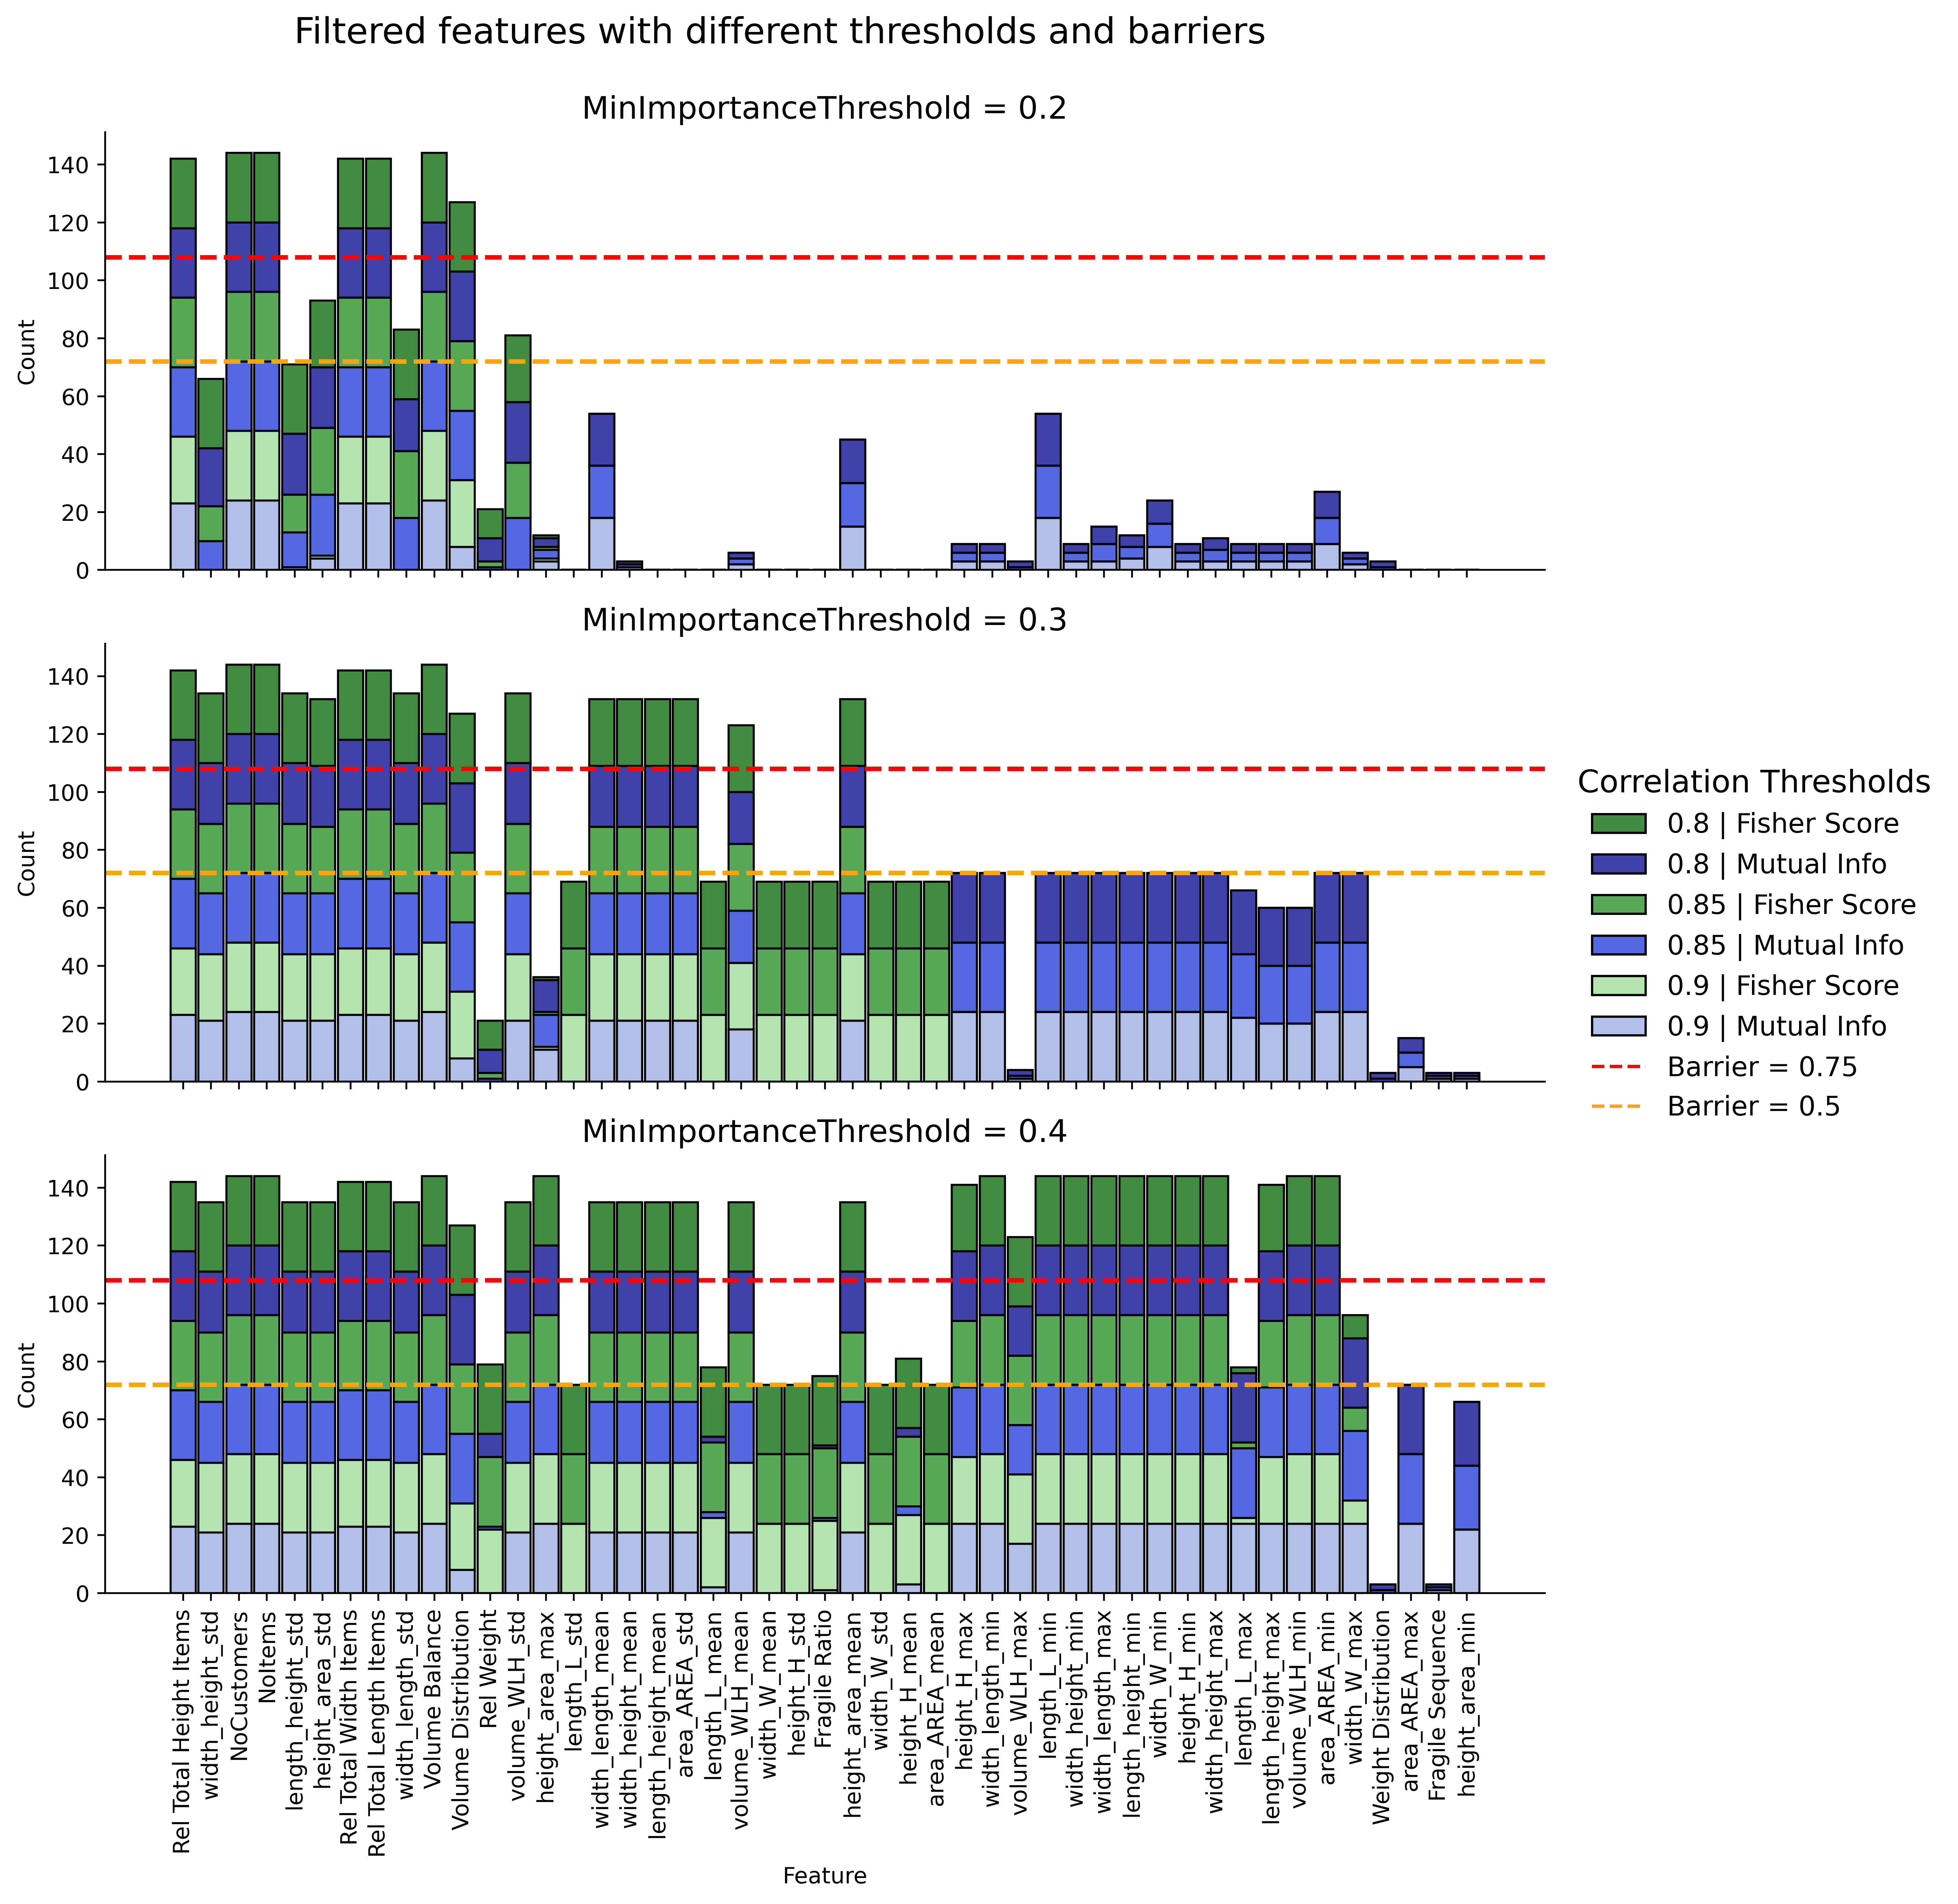
\includegraphics[width=\textwidth,height=0.75\textheight,keepaspectratio]{pictures/feature_filter_facePlot.png}
    \caption{Aggregated results from filter algorithm resulting in different drop sets.}
    \label{fig:feature_filter_parameters}
\end{figure}

\begin{table}[ht]
    \centering
    %\renewcommand{\arraystretch}{1.2}
    \rotatebox{90}{
        \footnotesize
        \begin{tabular}{@{}P{0.04\paperheight}P{0.04\paperheight}P{0.07\paperheight}P{0.05\paperheight}P{0.46\paperheight}@{}}
            \toprule
            Name         & Barrier $B$ & Importance Threshold $\epsilon$ & Number Features & Features                                                                                                                                                                                                                                                                                                                                                                                                                                                                                                                                                                                                                                                      \\
            \midrule
            DropSet-50-2 & 0.50        & 0.2                             & 10              & NoCustomers, NoItems, Rel Total Height Items, Rel Total Length Items, Rel Total Width Items, Volume Balance, Volume Distribution, height-area-std, volume-WLH-std, width-length-std                                                                                                                                                                                                                                                                                                                                                                                                                                                                           \\
            \midrule
            DropSet-50-3 & 0.50        & 0.3                             & 18              & NoCustomers, NoItems, Rel Total Height Items, Rel Total Length Items, Rel Total Width Items, Volume Balance, Volume Distribution, area-AREA-std, height-area-mean, height-area-std, length-height-mean, length-height-std, volume-WLH-mean, volume-WLH-std, width-height-mean, width-height-std, width-length-mean, width-length-std                                                                                                                                                                                                                                                                                                                          \\
            \midrule
            DropSet-50-4 & 0.50        & 0.4                             & 38              & Fragile Ratio, NoCustomers, NoItems, Rel Total Height Items, Rel Total Length Items, Rel Total Width Items, Rel Weight, Volume Balance, Volume Distribution, area-AREA-min, area-AREA-std, height-H-max, height-H-mean, height-H-min, height-area-max, height-area-mean, height-area-std, length-L-max, length-L-mean, length-L-min, length-height-max, length-height-mean, length-height-min, length-height-std, volume-WLH-max, volume-WLH-mean, volume-WLH-min, volume-WLH-std, width-W-max, width-W-min, width-height-max, width-height-mean, width-height-min, width-height-std, width-length-max, width-length-mean, width-length-min, width-length-std \\
            \midrule
            DropSet-75-2 & 0.50        & 0.2                             & 7               & NoCustomers, NoItems, Rel Total Height Items, Rel Total Length Items, Rel Total Width Items, Volume Balance, Volume Distribution                                                                                                                                                                                                                                                                                                                                                                                                                                                                                                                              \\
            \midrule
            DropSet-75-3 & 0.50        & 0.3                             & 18              & NoCustomers, NoItems, Rel Total Height Items, Rel Total Length Items, Rel Total Width Items, Volume Balance, Volume Distribution, area-AREA-std, height-area-mean, height-area-std, length-height-mean, length-height-std, volume-WLH-mean, volume-WLH-std, width-height-mean, width-height-std, width-length-mean, width-length-std                                                                                                                                                                                                                                                                                                                          \\
            \midrule
            DropSet-75-4 & 0.50        & 0.4                             & 32              & NoCustomers, NoItems, Rel Total Height Items, Rel Total Length Items, Rel Total Width Items, Volume Balance, Volume Distribution, area-AREA-min, area-AREA-std, height-H-max, height-H-min, height-area-max, height-area-mean, height-area-std, length-L-min, length-height-max, length-height-mean, length-height-min, length-height-std, volume-WLH-max, volume-WLH-mean, volume-WLH-min, volume-WLH-std, width-W-min, width-height-max, width-height-mean, width-height-min, width-height-std, width-length-max, width-length-mean, width-length-min, width-length-std                                                                                     \\

            \bottomrule
        \end{tabular}}
    \caption{Feature dropsets with different parameter combinations of $\epsilon$ and $B$.}
    \label{tab:feature_dropsets}
\end{table}

\begin{table}[ht]
    \centering
    \small
    \caption{Model hyperparameters for feature selection.}
    \label{tab:hyperparams_feature_selection}
    \renewcommand{\arraystretch}{1.1}
    \begin{tabular}{@{}c P{0.3\textwidth}P{0.3\textwidth}@{}}
        \toprule
        \textbf{LR}                  & \textbf{XGB}                    & \textbf{FFNN}                      \\
        \midrule
        \kv{penalty}{l2}             & \kv{objective}{binary:logistic} & \kv{hidden\_layers}{[128, 64, 32]} \\
        \kv{C}{1.0}                  & \kv{eval\_metric}{logloss}      & \kv{dropout}{0.2}                  \\
        \kv{solver}{lbfgs}           & \kv{max\_depth}{15}             & \kv{lr}{0.001}                     \\
        \kv{max\_iter}{1000}         & \kv{n\_estimators}{500}         & \kv{batch\_size}{512}              \\
        \kv{class\_weight}{balanced} & \kv{learning\_rate}{0.05}       & \kv{epochs}{50}                    \\
        \kv{random\_state}{42}       & \kv{subsample}{0.8}             & \kv{pos\_weight}{null}             \\
        \kv{n\_jobs}{23}             & \kv{colsample\_bytree}{0.8}     & \kv{weight\_decay}{0.0}            \\
                                     & \kv{reg\_alpha}{0.0}            & \kv{batch\_size}{512}              \\
                                     & \kv{reg\_lambda}{1.0}           & \kv{device}{cpu}                   \\
                                     & \kv{enable\_categorical}{false} & \kv{random\_state}{42}             \\
                                     & \kv{tree\_method}{hist}         & \kv{n\_jobs}{23}                   \\
                                     & \kv{n\_jobs}{23}                &                                    \\
                                     & \kv{random\_state}{42}          &                                    \\
        \bottomrule
    \end{tabular}
\end{table}

\clearpage
\section{Parking Lot}
\label{app:trash}
With a subset from krebs the following datasets were created!
\begin{table}[ht]
    \centering
    \begin{tabular}{c c cc c c c}
        \hline
        \makecell{Multiplier $\alpha$} & \makecell{Attempts                          \\ limit $\beta$} & \makecell{Success \\threshold $\gamma$} & Routes & Balance& \gls{MCC}-Score & F1-Score \\
        \hline
        1                              & 1                  & 1 & 7616  & 60/40 &  & \\
        1                              & 1                  & 2 & 15948 & 60/40 &  & \\
        1                              & 1                  & 3 & 24573 & 60/40 &  & \\
        1                              & 2                  & 1 & 8325  & 60/40 &  & \\
        1                              & 2                  & 2 & 17217 & 60/40 &  & \\
        1                              & 2                  & 3 & 26467 & 60/40 &  & \\
        1                              & 3                  & 1 & 8683  & 60/40 &  & \\
        1                              & 3                  & 2 & 18041 & 60/40 &  & \\
        1                              & 3                  & 3 & 27535 & 60/40 &  & \\
        \hline
    \end{tabular}
    \caption[Created instances for different parameter combinations $(\alpha, \beta, \gamma)$ for \krebsADataSetText dataset.]{Created instances for different parameter combinations $(\alpha, \beta, \gamma)$ for \krebsADataSetText dataset.
        The values in the balance column stand for the share of positive and netative labels in the sample population.}
    \label{tab:created_instances_xyz_krebs}
\end{table}



\begin{table}[ht]
    \centering
    \begin{tabular}{c c c c c c}
        \toprule
        Model                          & Name     & \gls{MCC}-Score & \gls{AUROC} & F1-Score & Accuracy \\
        \midrule
        \multirow{3}{*}{\gls{LR}}      & Complete & 0.6             & 0.9         & 0.87     & 0.95     \\
                                       & Trimmed  & 0.6             & 0.9         & 0.87     & 0.95     \\
                                       & Shrinked & 0.6             & 0.9         & 0.87     & 0.95     \\
        \midrule
        \multirow{3}{*}{Decision Tree} & Complete & 0.6             & 0.9         & 0.87     & 0.95     \\
                                       & Trimmed  & 0.6             & 0.9         & 0.87     & 0.95     \\
                                       & Shrinked & 0.6             & 0.9         & 0.87     & 0.95     \\
        \midrule
        \multirow{3}{*}{\gls{FFNN}}    & Complete & 0.6             & 0.9         & 0.87     & 0.95     \\
                                       & Trimmed  & 0.6             & 0.9         & 0.87     & 0.95     \\
                                       & Shrinked & 0.6             & 0.9         & 0.87     & 0.95     \\
        \bottomrule
    \end{tabular}
    \caption{Results}
    \label{tab:dataset_model_selection_saveStrategy}
\end{table}

\begin{table}[ht]
    \centering
    \begin{tabular}{c c c c c c}
        \toprule
        Model                           & Name       & \gls{MCC}-Score & \gls{AUROC} & F1-Score & Accuracy \\
        \midrule
        \multirow{13}{*}{\gls{LR}}      & RD-2-20-20 & 0.6             & 0.9         & 0.87     & 0.95     \\
                                        & RD-2-20-30 & 0.6             & 0.9         & 0.87     & 0.95     \\
                                        & RD-2-30-20 & 0.6             & 0.9         & 0.87     & 0.95     \\
                                        & RD-2-30-30 & 0.6             & 0.9         & 0.87     & 0.95     \\
                                        & RD-3-20-20 & 0.6             & 0.9         & 0.87     & 0.95     \\
                                        & RD-3-20-30 & 0.6             & 0.9         & 0.87     & 0.95     \\
                                        & RD-3-30-20 & 0.6             & 0.9         & 0.87     & 0.95     \\
                                        & RD-3-30-30 & 0.6             & 0.9         & 0.87     & 0.95     \\
                                        & RD-4-20-20 & 0.6             & 0.9         & 0.87     & 0.95     \\
                                        & RD-4-20-30 & 0.6             & 0.9         & 0.87     & 0.95     \\
                                        & RD-4-30-20 & 0.6             & 0.9         & 0.87     & 0.95     \\
                                        & RD-4-30-30 & 0.6             & 0.9         & 0.87     & 0.95     \\
                                        & RD-5-40-40 & 0.6             & 0.9         & 0.87     & 0.95     \\
        \midrule
        \multirow{13}{*}{Decision Tree} & RD-2-20-20 & 0.6             & 0.9         & 0.87     & 0.95     \\
                                        & RD-2-20-30 & 0.6             & 0.9         & 0.87     & 0.95     \\
                                        & RD-2-30-20 & 0.6             & 0.9         & 0.87     & 0.95     \\
                                        & RD-2-30-30 & 0.6             & 0.9         & 0.87     & 0.95     \\
                                        & RD-3-20-20 & 0.6             & 0.9         & 0.87     & 0.95     \\
                                        & RD-3-20-30 & 0.6             & 0.9         & 0.87     & 0.95     \\
                                        & RD-3-30-20 & 0.6             & 0.9         & 0.87     & 0.95     \\
                                        & RD-3-30-30 & 0.6             & 0.9         & 0.87     & 0.95     \\
                                        & RD-4-20-20 & 0.6             & 0.9         & 0.87     & 0.95     \\
                                        & RD-4-20-30 & 0.6             & 0.9         & 0.87     & 0.95     \\
                                        & RD-4-30-20 & 0.6             & 0.9         & 0.87     & 0.95     \\
                                        & RD-4-30-30 & 0.6             & 0.9         & 0.87     & 0.95     \\
                                        & RD-5-40-40 & 0.6             & 0.9         & 0.87     & 0.95     \\
        \midrule
        \multirow{13}{*}{\gls{FFNN}}    & RD-2-20-20 & 0.6             & 0.9         & 0.87     & 0.95     \\
                                        & RD-2-20-30 & 0.6             & 0.9         & 0.87     & 0.95     \\
                                        & RD-2-30-20 & 0.6             & 0.9         & 0.87     & 0.95     \\
                                        & RD-2-30-30 & 0.6             & 0.9         & 0.87     & 0.95     \\
                                        & RD-3-20-20 & 0.6             & 0.9         & 0.87     & 0.95     \\
                                        & RD-3-20-30 & 0.6             & 0.9         & 0.87     & 0.95     \\
                                        & RD-3-30-20 & 0.6             & 0.9         & 0.87     & 0.95     \\
                                        & RD-3-30-30 & 0.6             & 0.9         & 0.87     & 0.95     \\
                                        & RD-4-20-20 & 0.6             & 0.9         & 0.87     & 0.95     \\
                                        & RD-4-20-30 & 0.6             & 0.9         & 0.87     & 0.95     \\
                                        & RD-4-30-20 & 0.6             & 0.9         & 0.87     & 0.95     \\
                                        & RD-4-30-30 & 0.6             & 0.9         & 0.87     & 0.95     \\
                                        & RD-5-40-40 & 0.6             & 0.9         & 0.87     & 0.95     \\
        \bottomrule
    \end{tabular}
    \caption{Results}
    \label{tab:dataset_model_selection_randomStrategy}
\end{table}

\clearpage


\section{Parameterstudy}

\subsection{NoClasifier Variant}
\label{app:subsec:parameterstudy_noclassifier}

\begin{figure}[!ht]
    \centering
    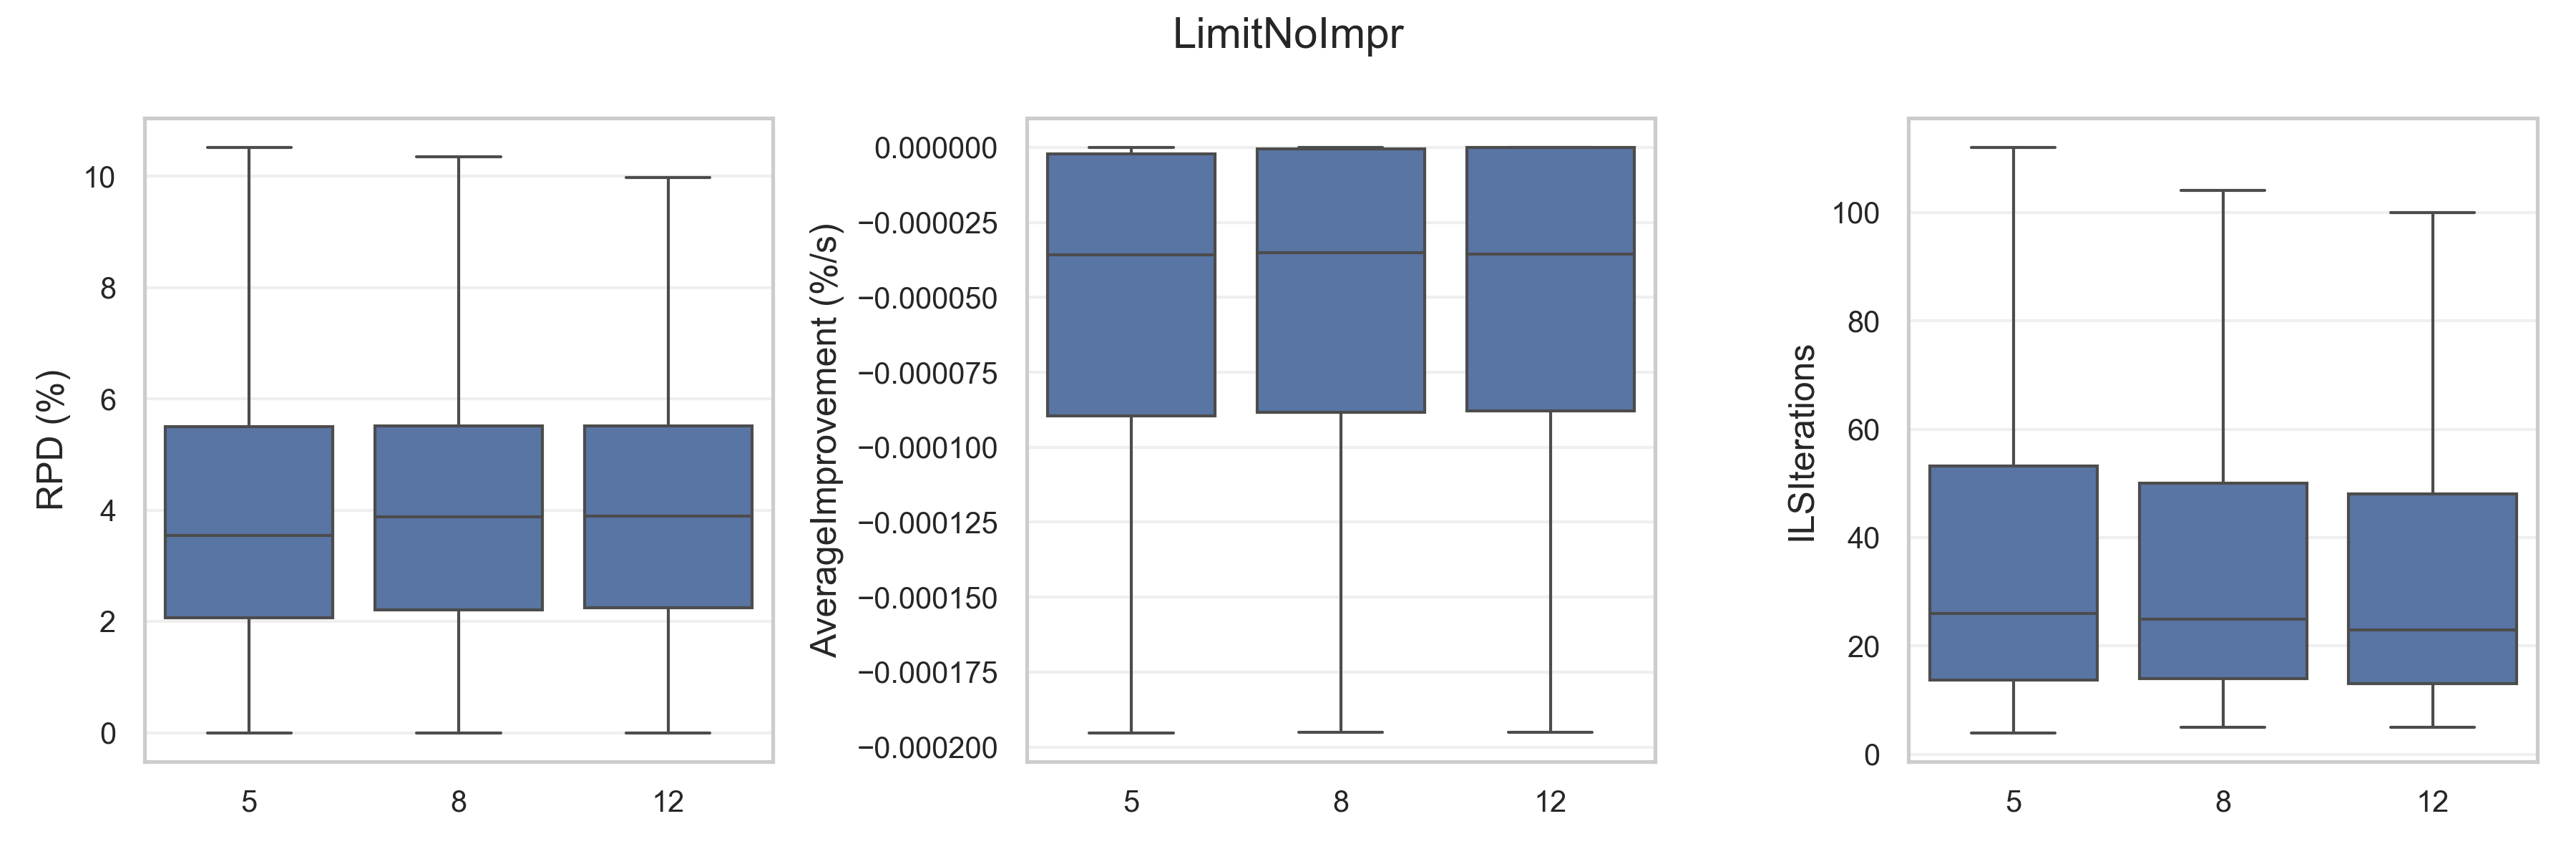
\includegraphics[width=\textwidth]{pictures/parameter_study/LimitNoImpr_base_parameter_study.png}
    \caption{Parameterstudy of LimitNoImpr divided in two groups based on the average iterations.}
    \label{fig:parameterstudy_NoClassifier_limitNoImpr}
\end{figure}

\begin{figure}[!ht]
    \centering
    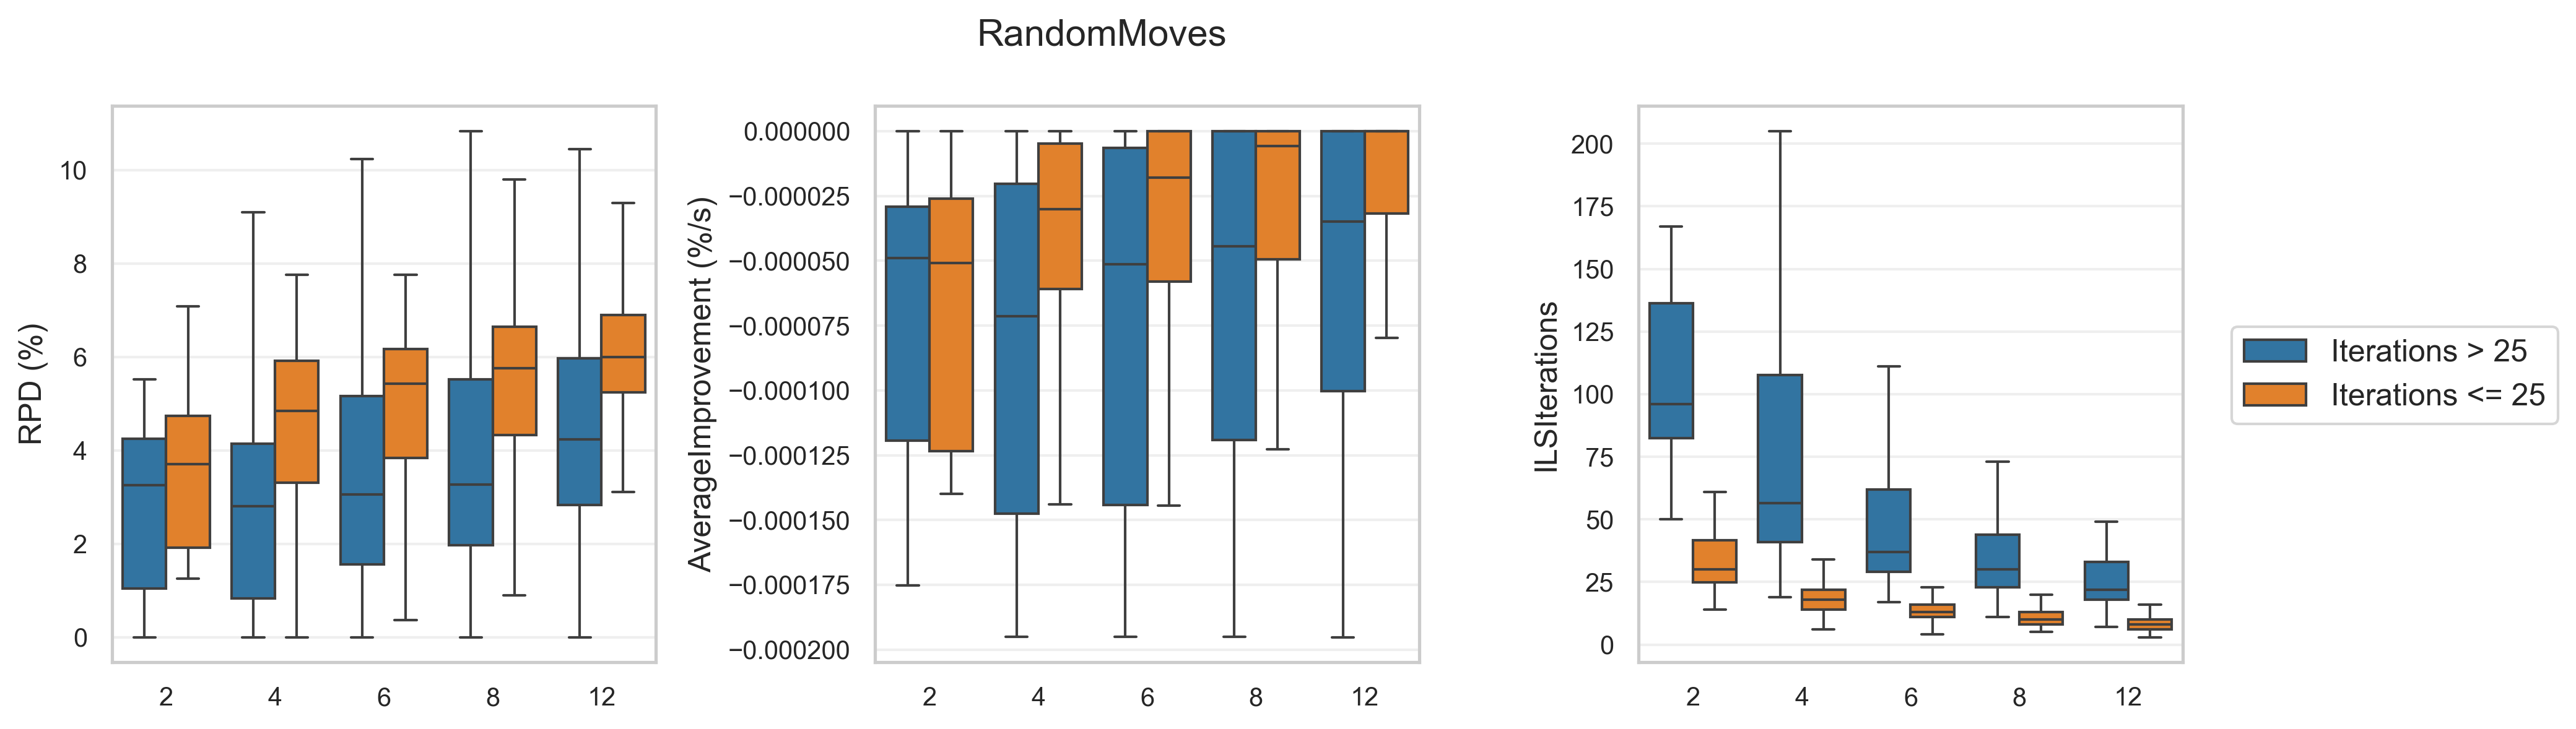
\includegraphics[width=\textwidth]{pictures/parameter_study/RandomMoves_base_parameter_study.png}
    \caption{Parameterstudy of RandomMoves divided in two groups based on the average iterations.}
    \label{fig:parameterstudy_NoClassifier_RandomMoves}
\end{figure}

\begin{figure}[!ht]
    \centering
    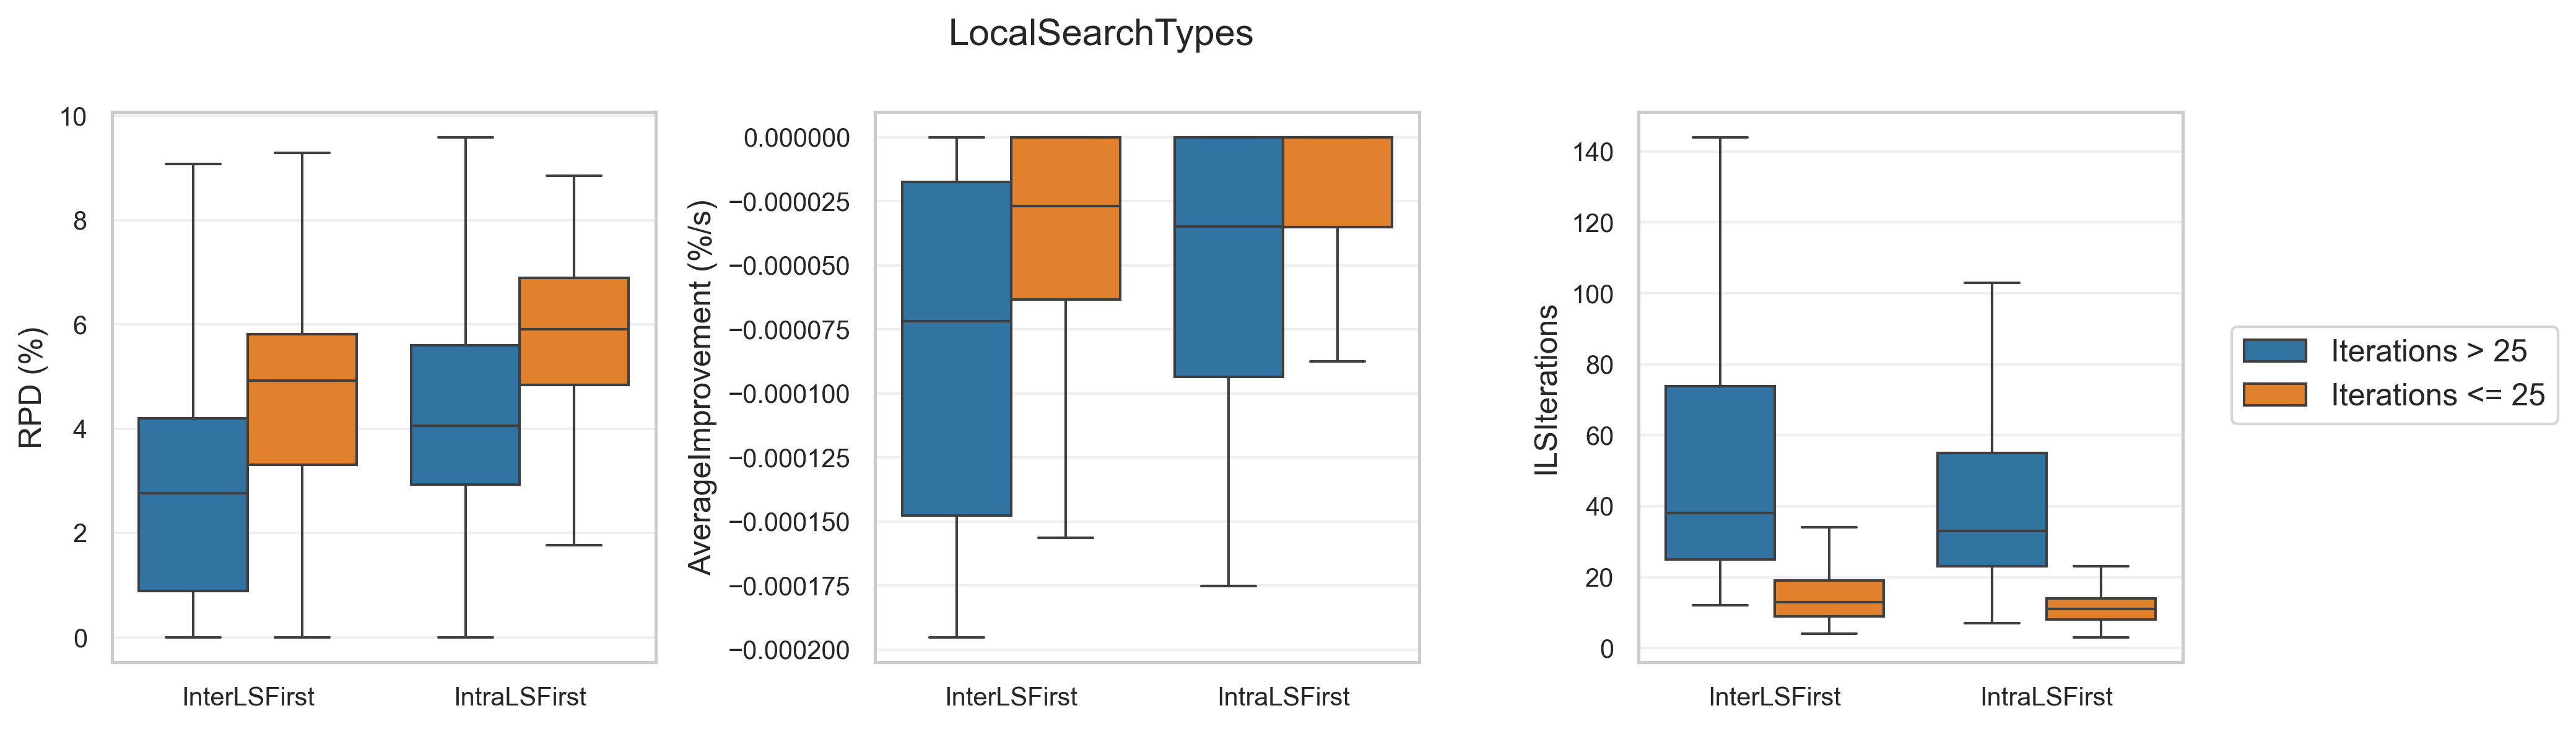
\includegraphics[width=\textwidth]{pictures/parameter_study/LocalSearchTypes_base_parameter_study.png}
    \caption{Parameterstudy of the order of local search neighborhoods divided in two groups based on the average iterations.}
    \label{fig:parameterstudy_NoClassifier_localSearch}
\end{figure}

\begin{figure}[!ht]
    \centering
    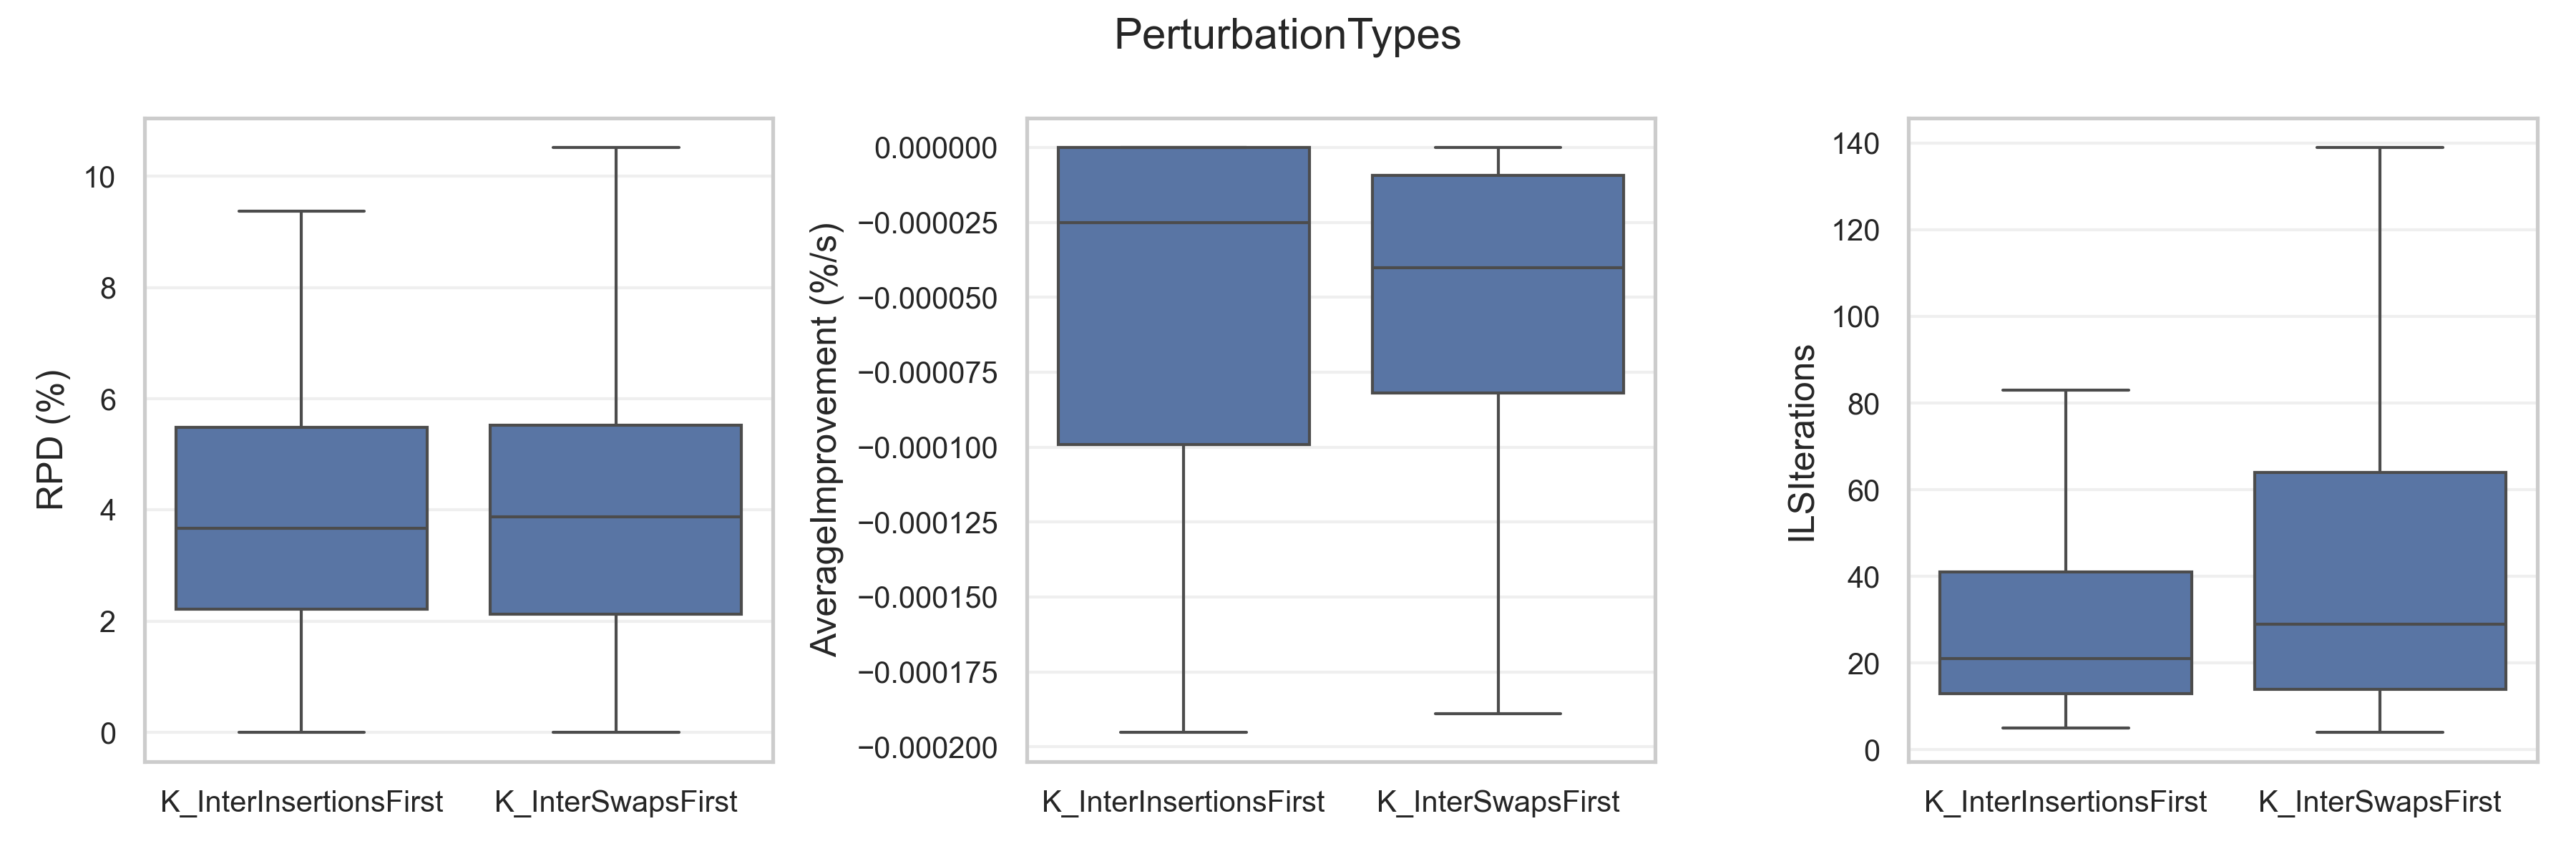
\includegraphics[width=\textwidth]{pictures/parameter_study/PerturbationTypes_base_parameter_study.png}
    \caption{Parameterstudy of the set and order of perturbation neighborhoods divided in two groups based on the average iterations.}
    \label{fig:parameterstudy_NoClassifier_perturbation}
\end{figure}

\subsection{SpeedUp Variant}
\label{app:subsec:parameterstudy_SpeedUp}

\section{Branch-and-Cut Results}

\begin{table}
    \centering
    \begin{tabular}{lrrrrl}
        \toprule
        Instance & Costs   & Gap  & NumberRoutes & $N$     & Runtime \\
        \midrule
        E016-03m & 301.66  & 0.00 & 4            & 4290    & 21      \\
        E016-05m & 334.96  & 0.00 & 5            & 53      & 1       \\
        E021-04m & 385.53  & 0.00 & 4            & 84225   & 532     \\
        E021-06m & 430.88  & 0.00 & 6            & 98      & 5       \\
        E022-04g & 427.56  & 0.00 & 5            & 138703  & 1024    \\
        E022-06m & 498.16  & 0.00 & 6            & 726     & 11      \\
        E023-03g & 757.88  & 0.00 & 5            & 1434923 & 4226    \\
        E023-05s & 798.65  & 0.01 & 6            & 2614340 & TL      \\
        E026-08m & 630.13  & 0.00 & 8            & 4604    & 61      \\
        E030-03g & 783.79  & 0.17 & 6            & 1153008 & TL      \\
        E030-04s & 728.32  & 0.16 & 7            & 1176116 & TL      \\
        E031-09h & 610.23  & 0.00 & 9            & 394216  & 10598   \\
        E033-03n & 2649.00 & 0.14 & 6            & 564692  & TL      \\
        E033-04g & 1337.17 & 0.25 & 7            & 432649  & TL      \\
        E033-05s & 1327.09 & 0.25 & 7            & 298863  & TL      \\
        E036-11h & 698.61  & 0.00 & 11           & 20025   & 325     \\
        E041-14h & 871.63  & 0.03 & 14           & 420758  & TL      \\
        E045-04f & 1204.07 & 0.18 & 10           & 306014  & TL      \\
        E051-05e & 726.20  & 0.19 & 10           & 305879  & TL      \\
        E072-04f & 567.64  & 0.24 & 15           & 162320  & TL      \\
        E076-07s & 1040.77 & 0.25 & 15           & 197632  & TL      \\
        E076-08s & 1134.70 & 0.26 & 16           & 222779  & TL      \\
        E076-10e & 1170.51 & 0.31 & 17           & 199955  & TL      \\
        E076-14s & 1121.85 & 0.13 & 16           & 168907  & TL      \\
        E101-08e & 1375.07 & 0.29 & 20           & 162886  & TL      \\
        E101-10c & 1544.02 & 0.28 & 22           & 229882  & TL      \\
        E101-14s & 1576.76 & 0.33 & 23           & 135945  & TL      \\
        \bottomrule
    \end{tabular}
    \caption{B\&C Results for obtaining save strategy dataset. Solution quality is presented by obj, gap (\%),
        and solution process metrics, including the total run time (TL = time limit) and explored branch-and-bound nodes $N$}
    \label{tab:bc_results_gendreau}
\end{table}

\clearpage
\section{\krebsADataSetText computational challenges}
\label{app:sec:krebs_computationally_challenges}

As shown in Table~\ref{tab:dataset_comparison}, an average route of \krebsADataSetText cotains four times more items than
in the \gendreauDataSet. This makes it much more computationally challenging to create a labeled train dataset with either
the \gls{CP} solver (random strategy) or by applying the B\&C algorithm (save strategy). When the two random datasets, RD-1-1-1-10
and RD-2-30-20-10, are compared. The difference bewteen the computation time for the \gls{CP} solver is huge. The average
\gls{CP} time for the dataset constructed from \krebsADataSetText is 247 seconds, but for \gendreauDataSetText only 0.244 seconds,
which is a factor of 1000. The following boxplot shows this dispersion of \gls{CP} times for each \gls{LST}.
\begin{figure}[ht]
    \centering
    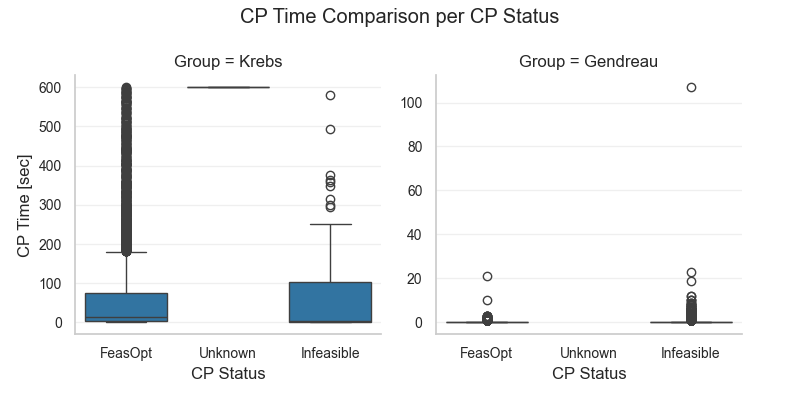
\includegraphics[width=0.8\textwidth]{pictures/comparison_krebs_gendreau/boxplot_cp_time.png}
    \caption{Boxplot showing the different computation times for \krebsADataSetText and \gendreauDataSet.}
    \label{fig:comparison_krebs_gendreau_boxplot}
\end{figure}

The time average difference is due to the group of routes labeled with \textit{Unknown} \gls{CP} status, which occurs, when
feasibility or infeasibility could not be proven in the maximum runtime of 600 seconds. From all routes from RD-1-1-1-10
33.6\% are classified as \textit{Unknown}. The distribution of \gls{LST} is shown in the following Figure~\ref{fig:comparison_krebs_gendreau_piechart}.

\begin{figure}[ht]
    \centering
    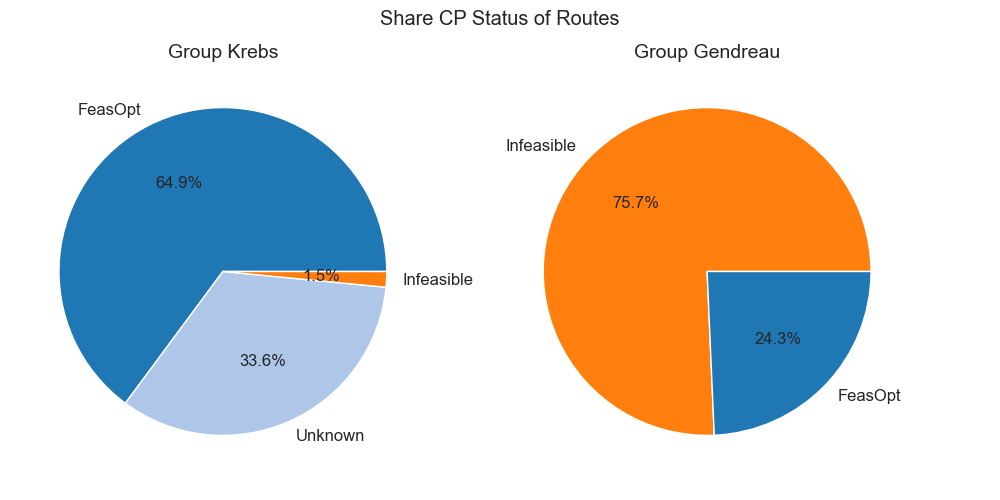
\includegraphics[width=0.8\textwidth]{pictures/comparison_krebs_gendreau/pie_chart_share_cp_status.png}
    \caption{Big share of unknown labeled tours for the \krebsADataSet.}
    \label{fig:comparison_krebs_gendreau_piechart}
\end{figure}
All routes classified as \textit{Unknown} will be consideres as \textit{Infeasible}, as outlined in Section~\ref{sec:DataRetrieval}. But
as the true label is not used, the model performance is weakened as possibly feasible routes will be labeled as infeasible. The
next Figure~\ref{fig:comparison_krebs_gendreau_numberItems} shows the effect of the number of items to the \gls{CP} time and the status.

\begin{figure}[ht]
    \centering
    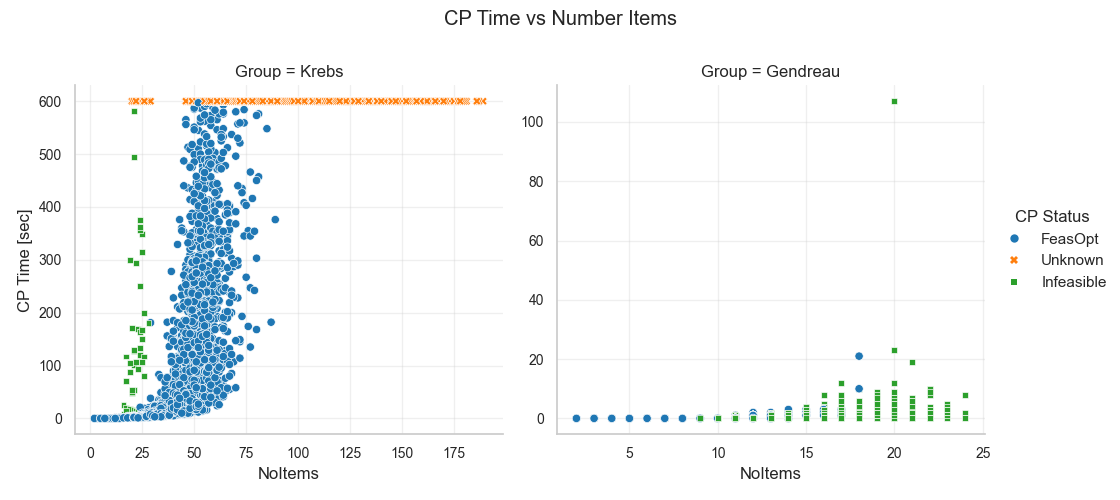
\includegraphics[width=0.8\textwidth]{pictures/comparison_krebs_gendreau/number_items_cp_status.png}
    \caption{Influence of number of items on the computational time.}
    \label{fig:comparison_krebs_gendreau_numberItems}
\end{figure}

The computation time literally explodes when more than 50 items are considered in a route, leading to an undefined \gls{CP} status, and
infeasible labels in the train dataset. So in the end, new long routes which improve the solution quality will always be classified as infeasible
or the exact computation time with the \gls{CP} solver takes too long to be used in a heuristic.
